
\section{Background and motivation}
\label{sec:background}

Fog infrastructures are distributed systems comprising heterogeneous
machines interconnected by communication links.

\begin{definition}[Fog infrastructure]
  A fog infrastructure is a \underline{g}raph $G(V, E)$ of
  \underline{v}ertices $V$ and bidirectional \underline{e}dges $E \in
  V \times V$. Edges have symmetric \underline{w}eights $w_{ij} =
  w_{ij}$ with $i, j \in V$.
\end{definition}

\begin{definition}[Logical partition]
  A logical \underline{p}artition $P_s$ originated at a
  \underline{s}ource process $s \in V$ is a set of interconnected
  processes that do not belong to another logical partition.
\end{definition}

\begin{definition}[Optimal partitioning]
  The optimal partitioning $\mathcal{P}$ is a set of logical
  partitions such that each process belongs to a logical partition
  comprising its closest source process. $\forall p \in P_{s_1},
  \nexists P_{s_2}$ such that \TODO{$distance(p, s_2) < distance(p,
    s_1)$}.
\end{definition}


\begin{figure*}
  \begin{center}
    \subfloat[Part A][\label{fig:addA}Both Process $a$ and
      Process $c$ initiate a partition.
      $w_{ab} = 1.5$; $w_{bc} = w_{cd} = w_{bd} = 1$.]{
\begin{tikzpicture}[scale=0.87]

  \thickmuskip=0mu
  \medmuskip=0mu
  \thinmuskip=0mu
  
  \newcommand\X{50pt}
  \newcommand\Y{-50pt}

  \newcommand\ADD{\alpha}


  
  \draw (-\X + 5pt, 0) --
  node[shape=circle, draw, fill=white, inner sep=0.5pt, font=\footnotesize]{2}
  (0 - 5pt, 0); %% a - b

  \draw (0 +5pt, 0) --
  node[shape=circle, draw, fill=white, inner sep=0.5pt, font=\footnotesize]{1}
  (\X -5pt, 0); %% b - c
  
  \draw (0, 0 - 5pt) --
  node[shape=circle, draw, fill=white, inner sep=0.5pt, font=\footnotesize]{1}
  (0, \Y + 5pt); %% d - b
  
  \draw (\X + 3pt, 0 - 5pt) --
  node[shape=circle, draw, fill=white, inner sep=0.5pt, font=\footnotesize]{3}
  (0 + 5pt, \Y - 3pt); %% c - d


  
  \draw[fill=white] (-\X, 0) node[color=\PA]{$\bm{a}$} +(-5pt, -5pt) rectangle +(5pt, 5pt);  
  \draw[fill=white] (0, 0) node{$\bm{b}$} +(-5pt, -5pt) rectangle +(5pt, 5pt);
  \draw[fill=white] (\X, 0) node{$\bm{c}$} +(-5pt, -5pt) rectangle +(5pt, 5pt);
  \draw[fill=white] (0, \Y) node[color=\PD]{$\bm{d}$} +(-5pt, -5pt) rectangle +(5pt, 5pt);
  
  \draw (-\X, 5pt) node[above, font=\small, color=\PA]{$\ADD_a^0$};
  \draw (-5pt, \Y) node[left, font=\small, color=\PD]{$\ADD_d^0$};

\end{tikzpicture}
}
    \hspace{5pt}
    \subfloat[Part B][\label{fig:addB}Messages transit through communication
      links and carry increasing weights.]{
\begin{tikzpicture}[scale=\SCALE]

  \thickmuskip=0mu
  \medmuskip=0mu
  \thinmuskip=0mu
  
  \newcommand\X{50pt}
  \newcommand\Y{-50pt}

  \newcommand\ADD{\alpha}


  
  \draw (-\X + 5pt, 0) --
  node[above=-0.3em, left=-0.3em, above left, font=\tiny]{$\textcolor{\PA}{\ADD_a^2} \rightarrow$}
  (0 - 5pt, 0); %% b - a 

  \draw (0 +5pt, 0) --
  (\X -5pt, 0); %% c - b

  \draw[opacity=0] (0, 0 - 5pt) --
  % node[opacity=1, above=-0.3em, font=\tiny, sloped]{$\textcolor{\PA}{\ADD_a^{3}} \rightarrow$}
  (0, \Y + 5pt); %% b - d
  \draw (0, \Y + 5pt) --
  node[above=-0.3em, font=\tiny, sloped]{$\textcolor{\PD}{\ADD_d^1} \rightarrow$}
  (0, 0 - 5pt);  %% d - b
  
  \draw (\X + 3pt, 0 - 5pt) --
  node[above=-0.3em, sloped, font=\tiny]{$\textcolor{\PD}{\ADD_{d}^{3}} \rightarrow$}
  (0 + 5pt, \Y - 3pt); %% c - d



  \draw[fill=white] (-\X, 0)
  node[color=\PA]{$\bm{a}$}
  +(-5pt, -5pt) rectangle +(5pt, 5pt);  
  \draw[fill=white] (0, 0) node{$\bm{b}$} +(-5pt, -5pt) rectangle +(5pt, 5pt);
  \draw[fill=white] (\X, 0) node{$\bm{c}$} +(-5pt, -5pt) rectangle +(5pt, 5pt);
  \draw[fill=white] (0, \Y) node[color=\PD]{$\bm{d}$} +(-5pt, -5pt) rectangle +(5pt, 5pt);
  
  \draw (-\X, 5pt) node[above, font=\small, color=\PA]{$\ADD_a^0$};
  \draw (-5pt, \Y) node[left, font=\small, color=\PD]{$\ADD_d^0$};

\end{tikzpicture}
}
    \hspace{5pt}
    \subfloat[Part C][\label{fig:addC}Process $b$ receives and forwards
      $Add_{c, 1}$ then discards $Add_{a, 1.5}$, for the latter distance
      is higher.]{
\begin{tikzpicture}[scale=\SCALE]

  \draw (-\X + 5pt, 0) --
  node[above=-0.3em, right=-0.5em, above right, font=\SMSG]{$\textcolor{\PA}{\alpha_a^2} \RIGHT$}
  node[below=-0.3em, font=\SMSG]{$\LEFT \textcolor{\PD}{\alpha_d^3}$}
  (0 - 5pt, 0); %% b - a 

  \draw (0 +5pt, 0) --
  node[above=-0.3em, font=\SMSG]{$\LEFT \textcolor{\PD}{\alpha_d^4}$}  
  node[below=-0.3em, font=\SMSG]{$\textcolor{\PD}{\alpha_d^2} \RIGHT$}  
  (\X -5pt, 0); %% b - c

  \draw[opacity=0] (0, 0 - 5pt) --
  node[opacity=\OACK, above=-0.3em, sloped, font=\SMSG]{$\alpha_d^2 \RIGHT$}
  (0, \Y + 5pt); %% b - d
  \draw[->] (0, \Y + 5pt) --
  (0, 0 - 5pt);  %% d - b
  
  \draw[<-] (\X + 3pt, 0 - 5pt) --
  node[opacity=\OACK, below=-0.3em, sloped, font=\SMSG]{$\LEFT \alpha_d^6$}
  (0 + 5pt, \Y - 3pt); %% c - d


  
  \draw[fill=white] (-\X, 0)
  node[color=\PA]{$\bm{a}$}
  +(-5pt, -5pt) rectangle +(5pt, 5pt);  
  \draw[fill=white] (0, 0)
  node[color=\PC]{$\bm{b}$}
  +(-5pt, -5pt) rectangle +(5pt, 5pt);
  \draw[fill=white] (\X, 0)
  node[color=\PC]{$\bm{c}$}
  +(-5pt, -5pt) rectangle +(5pt, 5pt);
  \draw[fill=white] (0, \Y)
  node[color=\PC]{$\bm{d}$}
  +(-5pt, -5pt) rectangle +(5pt, 5pt);

  \draw ( 0, 5pt) node[above, font=\small, color=\PD]{$\alpha_d^1$}; % b
  \draw ( \X, 5pt) node[above, font=\small, color=\PD]{$\alpha_d^3$}; % c
  \draw (-\X, 5pt) node[above, font=\small, color=\PA]{$\alpha_a^0$}; % a
  \draw (-5pt, \Y) node[left, font=\small, color=\PD]{$\alpha_d^0$}; % d
  
\end{tikzpicture}
}
    \hspace{5pt}
    \subfloat[Part D][\label{fig:addD}Processes $b$, $c$, and $d$ discard
      incoming messages. The system converged to optimal partitions.]{
      
\begin{tikzpicture}[scale=\SCALE]

  \thickmuskip=0mu
  \medmuskip=0mu
  \thinmuskip=0mu
  
  \newcommand\X{50pt}
  \newcommand\Y{-50pt}

  \newcommand\ADD{\alpha}


  
  \draw (-\X + 5pt, 0) -- (0 - 5pt, 0); %% a - b

  \draw (0 +5pt, 0) --
  (\X -5pt, 0); %% b - c

  \draw (0, \Y + 5pt) --
  (0, 0 - 5pt);  %% d - b
  
  \draw (\X + 3pt, 0 - 5pt) --
  node[below=-0.3em, sloped, font=\tiny]{$\LEFT \textcolor{\PD}{\ADD_{d}^{5}}$}
  (0 + 5pt, \Y - 3pt); %% c - d


  
  \draw[fill=white] (-\X, 0)
  node[color=\PA]{$\bm{a}$}
  +(-5pt, -5pt) rectangle +(5pt, 5pt);  
  \draw[fill=white] (0, 0)
  node[color=\PC]{$\bm{b}$}
  +(-5pt, -5pt) rectangle +(5pt, 5pt);
  \draw[fill=white] (\X, 0)
  node[color=\PC]{$\bm{c}$}
  +(-5pt, -5pt) rectangle +(5pt, 5pt);
  \draw[fill=white] (0, \Y)
  node[color=\PC]{$\bm{d}$}
  +(-5pt, -5pt) rectangle +(5pt, 5pt);
  
  \draw ( 0, 5pt) node[above, font=\small, color=\PD]{$\ADD_d^1$}; % b
  \draw ( \X, 5pt) node[above, font=\small, color=\PD]{$\ADD_d^2$}; % c
  \draw (-\X, 5pt) node[above, font=\small, color=\PA]{$\ADD_a^0$}; % a
  \draw (-5pt, \Y) node[left, font=\small, color=\PD]{$\ADD_d^0$}; % d

  
\end{tikzpicture}
}
    \caption{\label{fig:add}Simple accumulation in messages makes the
      system converge to optimal partitions with contained
      broadcast.}
  \end{center}
\end{figure*}

\begin{algorithm}
  \SetKwProg{Function}{func}{}{}

\small

\DontPrintSemicolon
\LinesNumbered

$O_p$, $W_p$\tcp*[r]{set of neighbors and weights}
$s \leftarrow \varnothing$ \tcp*[r]{best source of partition ($\sigma$)}
$d \leftarrow \infty$ \tcp*[r]{smallest distance to $s$ ($\sigma$ and $\mu$)}


\BlankLine

\Function{\textup{Add ( )} \tcp*[f]{$\alpha_p^0$}} {
  \textup{receiveAdd($\varnothing$, $p$, $0$)} \label{line:lowestbound} \tcp*[f]{$b_p(\alpha_p^0)$}
}

\BlankLine

\Function{\textup{receiveAdd($q$, $s'$, $d'$)} \tcp*[f]{$r_p(\alpha_{s'}^{d'})$ from $q$}} {
  \If (\tcp*[f]{($\phi$)}){$d' < d$} {
      $s \leftarrow s'$ \tcp*[r]{\smash{$d_p(\alpha_{s'}^{d'})$}}
      $d \leftarrow d'$ \;

      \ForEach(\tcp*[f]{\smash{$f_p(\alpha_{s'}^{d'})$}}) {$n \in O_p \setminus q$} {
          \textup{send$_n$($s', d' + W_{pn}$)} \label{line:accumulator}
          \tcp*[r]{\smash{$s_{pn}(\alpha_{s'}^{d'+w_{pn}})$}}
       }      
  }
}

%% \BlankLine

%% \Function{\textup{edgeUp($q$)} \tcp*[f]{new link to $q$}} {
%%   \lIf { $d < \infty$} {\textup{send$_q$($s, d + W_{pq}$)}}
%% }



  \caption{\label{algo:add}Adding a partition by Process $p$.}
\end{algorithm}

When $distance$ involves monotonically increasing scalars such as
latency or number of hops between sources and processes, the optimal
partitioning consists in processing the multiple destinations shortest
path~\REF at each process.  Algorithm~\ref{algo:add} shows the
instructions of such dynamic partitioning where the only operation
available to processes is the adding of a
partition. Figure~\ref{fig:add} illustrates its behavior on a system
comprising 4 processes $a$, $b$, $c$, and $d$. Two processes $a$ and
$c$ concurrently create a partition. They initialize their own state
with the lowest possible bound $0$ (see Line~\ref{line:lowestbound}),
and send a message to each of their neighbors by accumulating the
corresponding edge weight (see Line~\ref{line:accumulator}). In
Figure~\ref{fig:addC}, Process $b$ receives $Add_{c, 1}$. Since it
improves its own partition distance, it keeps it and forwards it to
its neighbors. Process $b$ discards $Add_{b, 1.5}$, for it does not
improve its partition distance. Processes $c$ and $d$ will never hear
of Process $a$'s partition. \TODO{At scale.} In Figure~\ref{fig:addD},
processes discard last transiting messages. The system converged to
the optimal partitioning.

Transitive relationships ensure that each process gets its closest
source while accumulators ensure that messages propagation
terminates. The system converges towards the optimal partitioning
despite processes not broadcasting all messages. Removals of
partitions are more challenging. \TODO{Figure.} \TODO{Also easy to
  solve when all processes receive all messages}. One could solve this
issue by removing partitions that were not advertised for a defined
time~\REF. However, relying on physical timeout could lead to either
premature removals of partitions when they are still operating; or
slow convergence where processes believe they belong to a partition
that was removed.


\begin{figure*}
  \begin{center}
    \subfloat[Part A][\label{fig:delA}Both Process $a$ and
      Process $c$ initiate then remove a partition.
      $w_{ab} = 1.5$; $w_{bc} = w_{cd} = w_{bd} = 1$.]{
\begin{tikzpicture}[scale=\SCALE]

  \draw[opacity=0](-2.45*\X, 0) -- (2.45*\X, 0); %% more space for caption
  

  
  \draw (-\X + 5pt, 0) --
  node[above=-0.3em,font=\tiny]{$\DEL_{a} \RIGHT$}
  (0 - 5pt, 0); %% b - a 

  \draw (0 +5pt, 0) --
  (\X -5pt, 0); %% b - c

  \draw [<-] (0, 0 - 5pt) --
  (0, \Y + 5pt);  %% b - d
  
  \draw [<-] (\X + 3pt, 0 - 5pt) --
  (0 + 5pt, \Y - 3pt); %% c - d


  
  \draw[fill=white] (-\X, 0) node{$\bm{a}$} +(-5pt, -5pt) rectangle +(5pt, 5pt);  
  \draw[fill=white] (0, 0) node[color=\PD]{$\bm{b}$} +(-5pt, -5pt) rectangle +(5pt, 5pt);
  \draw[fill=white] (\X, 0) node[color=\PD]{$\bm{c}$} +(-5pt, -5pt) rectangle +(5pt, 5pt);
  \draw[fill=white] (0, \Y) node[color=\PD]{$\bm{d}$} +(-5pt, -5pt) rectangle +(5pt, 5pt);
  
  \draw (-\X, 5pt) node[above, font=\small]{$\DEL_a$};
  \draw (0, 5pt) node[above, font=\small, color=\PD]{$\ADD_d^1$};
  \draw (\X, 5pt) node[above, font=\small, color=\PD]{$\ADD_d^2$};
  \draw (-5pt, \Y) node[left, font=\small, color=\PD]{$\ADD_d^0$};


\end{tikzpicture}
}
    \hspace{5pt}
    \subfloat[Part B][\label{fig:delB}Process $b$ and Process $d$ receive and deliver
      messages based on their weights. $a$'s partition propagates to all processes.]
             {
\begin{tikzpicture}[scale=0.87]

  \thickmuskip=0mu
  \medmuskip=0mu
  \thinmuskip=0mu
  
  \newcommand\X{50pt}
  \newcommand\Y{-50pt}

  \newcommand\ADD{\alpha}
  \newcommand\DEL{\delta}



  \draw (-\X + 5pt, 0) --
  node[above=-0.3em,font=\tiny]{$\DEL_{a} \rightarrow$}
  node[below=-0.3em,font=\tiny]{$\leftarrow \ADD_{a}^{3}$}
  (0 - 5pt, 0); %% b - a 

  \draw (0 +5pt, 0) --
  node[above=-0.3em, font=\tiny]{$\leftarrow \textcolor{\PC}{\ADD_{c}^{1}}\cdot\DEL{c}$}
  node[below=-0.3em, font=\tiny]{$\textcolor{\PA}{\ADD_a^{2.5}} \rightarrow$}
  (\X -5pt, 0); %% b - c

  \draw[opacity=0] (0, 0 - 5pt) --
  node[opacity=1, above=-0.3em, font=\tiny, sloped]{$\ADD_a^{2.5} \rightarrow$}
  (0, \Y + 5pt); %% b - d
  \draw (0, \Y + 5pt) --
  node[above=-0.3em, font=\tiny, sloped]{$\ADD_c^2 \rightarrow$}
  (0, 0 - 5pt);  %% d - b
  
  \draw (\X + 3pt, 0 - 5pt) --
  node[above=-0.3em, font=\tiny, sloped]{$\ADD_{c}^{2} \rightarrow$}
  node[below=-0.3em, font=\tiny, sloped]{$\leftarrow \DEL_c$}
  (0 + 5pt, \Y - 3pt); %% c - d



  
  \draw[fill=white] (-\X, 0) node{$\bm{a}$} +(-5pt, -5pt) rectangle +(5pt, 5pt);  
  \draw[fill=white] (0, 0) node[color=\PA]{$\bm{b}$} +(-5pt, -5pt) rectangle +(5pt, 5pt);
  \draw[fill=white] (\X, 0) node{$\bm{c}$} +(-5pt, -5pt) rectangle +(5pt, 5pt);
  \draw[fill=white] (0, \Y) node[color=\PC]{$\bm{d}$} +(-5pt, -5pt) rectangle +(5pt, 5pt);
  
  % \draw (-\X+5pt, 5pt) node[above left]{$\DEL_a$};
  % \draw (\X+5pt, 5pt) node[above right]{$\DEL_c$};
  \draw (0, 5pt) node[above]{$\bm{a: 1.5}$};
  \draw (-5pt, \Y) node[left]{$\bm{c: 1}$};


\end{tikzpicture}
}
    \hspace{5pt}
    \subfloat[Part C][\label{fig:delC}Process $c$'s partition reach $b$ and $d$.
      Its removal shortly follows. Process $b$ does not have any control
      information about partitions any more.]{
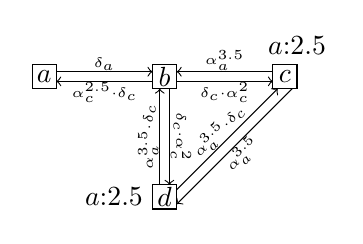
\begin{tikzpicture}[scale=0.87]

  \newcommand\X{50pt}
  \newcommand\Y{-50pt}

  \newcommand\ADD{\alpha}
  \newcommand\DEL{\delta}

  \thickmuskip=0mu
  \medmuskip=0mu
  \thinmuskip=0mu

  \draw[->] (-\X + 5pt, 0 + 2pt ) --
  node[above=-0.3em,font=\tiny]{$\bm{\DEL_{a}}$}
  (0 - 5pt, 0 + 2pt); %% a - b
  \draw[<-] (-\X + 5pt, 0 - 2pt ) --
  node[below=-0.3em,font=\tiny]{$\ADD_{c}^{2.5}\cdot\DEL_{c}$}
  (0 - 5pt, 0 - 2pt); %% b - a 

  \draw[<-] (0 +5pt, 0 + 2pt) --
  node[above=-0.3em, font=\tiny]{$\ADD_a^{3.5}$}
  (\X -5pt, 0 + 2pt); %% c - b
  \draw[->] (0 +5pt, 0 - 2pt) --
  node[below=-0.3em, font=\tiny]{$\DEL_{c}\cdot\ADD_c^{2}$}
  (\X -5pt, 0 - 2pt); %% b - c

  \draw[->] (0 + 2pt, 0 - 5pt) --
  node[above=-0.3em, font=\tiny, sloped]{$\DEL_{c}\cdot\ADD_c^{2}$}
  (0 + 2pt, \Y + 5pt); %% b - d
  \draw[->] (0 - 2pt, \Y + 5pt) --
  node[above=-0.3em, font=\tiny, sloped]{$\ADD_{a}^{3.5}\cdot\DEL_c$}
  (0 - 2pt, 0 - 5pt);  %% d - b
  
  \draw[<-] (\X - 3pt, 0 - 5pt) --
  node[above=-0.3em, font=\tiny, sloped]{$\ADD_{a}^{3.5}\cdot\DEL_{c}$}
  (0 + 5pt, \Y + 3pt); %% d - c
  \draw[->] (\X + 3pt, 0 - 5pt) --
  node[below=-0.3em, font=\tiny, sloped]{$\ADD_{a}^{3.5}$}
  (0 + 5pt, \Y - 3pt); %% c - d



  
  \draw[fill=white] (-\X, 0) node{$\bm{a}$} +(-5pt, -5pt) rectangle +(5pt, 5pt);  
  \draw[fill=white] (0, 0) node{$\bm{b}$} +(-5pt, -5pt) rectangle +(5pt, 5pt);
  \draw[fill=white] (\X, 0) node{$\bm{c}$} +(-5pt, -5pt) rectangle +(5pt, 5pt);
  \draw[fill=white] (0, \Y) node{$\bm{d}$} +(-5pt, -5pt) rectangle +(5pt, 5pt);
  
  % \draw (-\X+5pt, 5pt) node[above left]{$\DEL_a$};
  \draw (\X+5pt, 5pt) node[above]{$\bm{a: 2.5}$}; %% c
  % \draw (0, 5pt) node[above]{$\bm{a: 1.5}$}; %% b
  \draw (-5pt, \Y) node[left]{$\bm{a: 2.5}$}; %% d


\end{tikzpicture}
}
    \hspace{5pt}
    \subfloat[Part D][\label{fig:delD}Processes discard remaining messages.
      Process $b$ does not deliver $\delta_a$, for it already removed $a$ when
      Partition $c$ dominated it. Processes $c$ and $d$ remain in an incorrect
      partition.]{
\begin{tikzpicture}[scale=0.87]

  \newcommand\X{50pt}
  \newcommand\Y{-50pt}

  \newcommand\ADD{\alpha}
  \newcommand\DEL{\delta}

  \thickmuskip=0mu
  \medmuskip=0mu
  \thinmuskip=0mu

  \draw[->] (-\X + 5pt, 0 + 2pt ) --
  node[above=-0.3em,font=\tiny]{$\DEL{c}\cdot\ADD_c^{4}\cdot$\textcolor{\WRONG}{$\bm{\DEL_{a}}$}}
  (0 - 5pt, 0 + 2pt); %% a - b
  \draw[<-] (-\X + 5pt, 0 - 2pt ) --
  (0 - 5pt, 0 - 2pt); %% b - a 

  \draw[<-] (0 +5pt, 0 + 2pt) --
  (\X -5pt, 0 + 2pt); %% c - b
  \draw[->] (0 +5pt, 0 - 2pt) --
  (\X -5pt, 0 - 2pt); %% b - c

  \draw[->] (0 + 2pt, 0 - 5pt) --
  (0 + 2pt, \Y + 5pt); %% b - d
  \draw[->] (0 - 2pt, \Y + 5pt) --
  (0 - 2pt, 0 - 5pt);  %% d - b
  
  \draw[<-] (\X - 3pt, 0 - 5pt) --
  (0 + 5pt, \Y + 3pt); %% d - c
  \draw[->] (\X + 3pt, 0 - 5pt) --
  (0 + 5pt, \Y - 3pt); %% c - d



  
  \draw[fill=white] (-\X, 0) node{$\bm{a}$} +(-5pt, -5pt) rectangle +(5pt, 5pt);  
  \draw[fill=white] (0, 0)
  node[color=\WRONG]{$\bm{b}$} +(-5pt, -5pt)
  rectangle +(5pt, 5pt);
  \draw[fill=white] (\X, 0) node{$\bm{c}$} +(-5pt, -5pt) rectangle +(5pt, 5pt);
  \draw[fill=white] (0, \Y) node{$\bm{d}$} +(-5pt, -5pt) rectangle +(5pt, 5pt);
  
  % \draw (-\X+5pt, 5pt) node[above left]{$\DEL_a$};
  \draw (\X+5pt, 5pt) node[above, color=\WRONG]{$\bm{a: 2.5}$}; %% c
  % \draw (0, 5pt) node[above]{$\bm{a: 1.5}$}; %% b
  \draw (-5pt, \Y) node[left, color=\WRONG]{$\bm{a: 2.5}$}; %% d


\end{tikzpicture}
}
  \end{center}
  \caption{\label{algo:add}Removing partition may lead to inconsistent states.}
\end{figure*}



Order on the broadcast.

\TODO{Problem statement.}

\TODO{Next Section presents our approach that solves this problem
  statement by relying only on logical control information.}

%%% Local Variables: 
%%% mode: latex
%%% TeX-master: "../paper"
%%% ispell-local-dictionary: "english"
%%% End: 

